\section{Methods}
\label{sec:method}


\begin{figure}[!htbp]
\centering
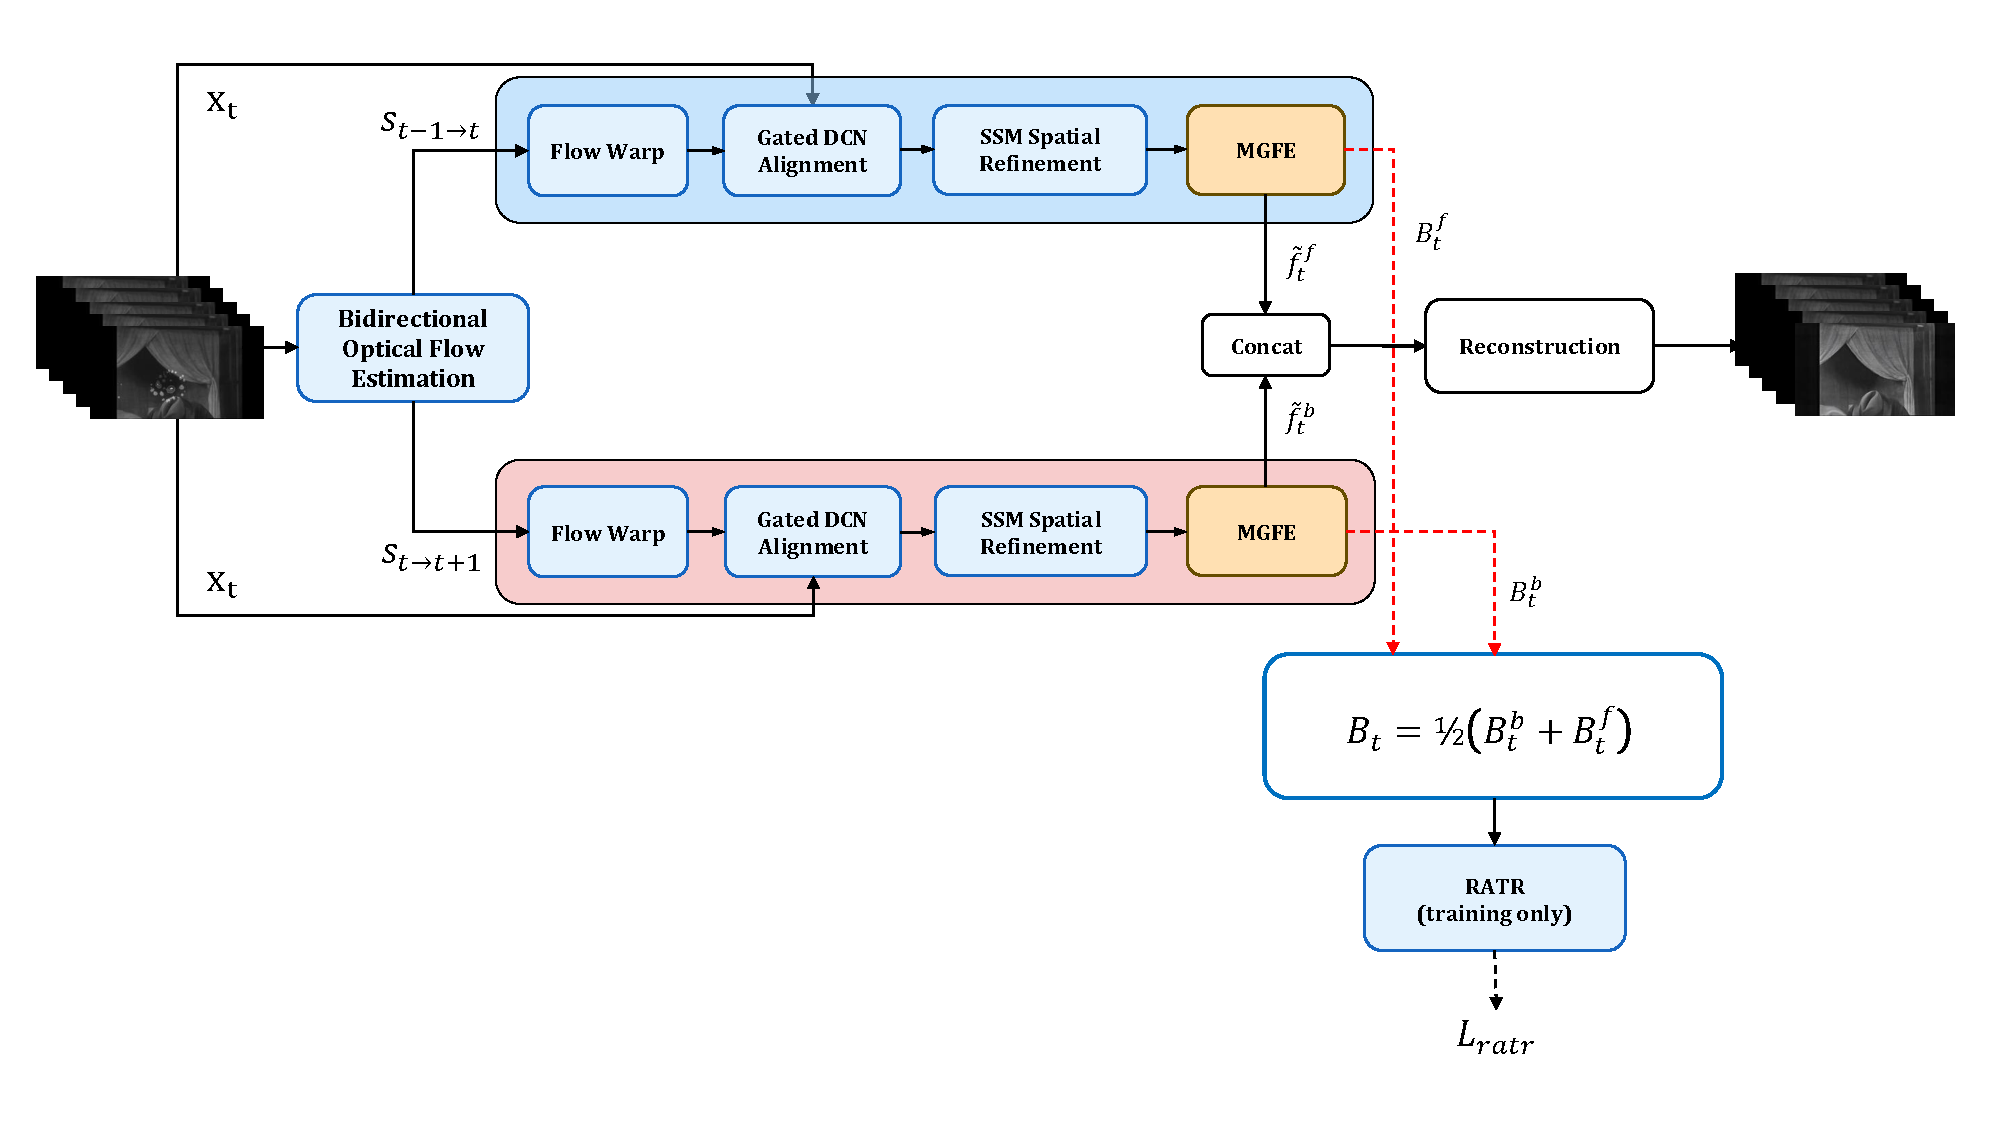
\includegraphics[width=\textwidth]{figures/Fig1_mgfrofr_architecture.pdf}
\caption{MgfrOFR framework. MGFE decomposes propagated features into $G{=}3$ multi-granularity restoration-token branches and uses their summaries for channel-wise recalibration. RATR is used only during training (dashed red path) to penalize redundant temporal-ranking correlations and produce $\mathcal{L}_{\text{intra}}$ and $\mathcal{L}_{\text{inter}}$.\label{fig:architecture}}
\end{figure}

\subsection{Problem Setup}
\label{subsec:problem_setup}

Given a degraded old-film clip $X=\{x_t\}_{t=1}^{T}$, the task is to estimate a restored clip $Y=\{y_t\}_{t=1}^{T}$ that recovers image content while suppressing structured film defects and photometric degradation. Synthetic SRWOV samples provide paired clean frames for direct supervision. Real-world archival clips do not provide ground truth, so their evaluation relies on no-reference quality metrics and qualitative inspection. The method must therefore preserve temporal consistency while handling degradations that vary across both spatial scale and time.

\subsection{Input Representation}
\label{subsec:input_representation}

MgfrOFR operates on the propagated feature maps produced by the baseline bidirectional restoration backbone. For each time step $t$, the backward and forward streams produce aligned feature maps $f_t^{b}, f_t^{f} \in \mathbb{R}^{C_f \times H \times W}$ after motion-aware propagation. MgfrOFR treats these maps as the only interface to the backbone: MGFE reads each propagated map, returns a recalibrated map with the same spatial size and channel count, and emits branch descriptors used by RATR during training.

MgfrOFR follows the same bidirectional propagation framework as MambaOFR~\cite{mao2025mambaofr} while adding an explicit coarse-to-fine representation pipeline. Given a degraded input clip $X=\{x_t\}_{t=1}^{T}$, the baseline first propagates content in backward and forward directions so that neighboring observations are motion-aligned before reconstruction. MgfrOFR then separates restoration evidence by spatial granularity and regularizes the resulting branches during training. In the representation-level symmetry framing used here, coarse, medium, and fine restoration evidence should remain balanced even when the input damage is spatially and temporally asymmetric.

The two added components serve different roles. MGFE converts each propagated feature map into a token sequence, inserts learnable restoration tokens, derives branch descriptors from progressively fused token groups, and feeds their summaries back through channel-wise recalibration. RATR is used only during training; it discourages redundant ranking behavior across branches and does not add an inference module. The reconstruction head follows the original MambaOFR contract and outputs the restored frame. The overall architecture is illustrated in Figure~\ref{fig:architecture}.

\begin{algorithm}[H]
\caption{MgfrOFR forward pass for a clip of length $T$.\label{alg:mgfrofr}}
\begin{algorithmic}[1]
\Require Degraded clip $X=\{x_t\}_{t=1}^{T}$
\Ensure Restored frames $\{y_t\}_{t=1}^{T}$
\State Initialize descriptor buffer $\mathcal{B} \leftarrow \emptyset$
\For{$t = 1$ to $T$}
    \State $f_t^{b}, f_t^{f} \leftarrow \text{Backbone}(X, t)$ \Comment{Bidirectional propagation}
    \For{$d \in \{b, f\}$}
        \State $\widetilde{f}_t^{d}, B_t^{d} \leftarrow \text{MGFE}(f_t^{d})$ \Comment{Multi-granularity decomposition}
    \EndFor
    \State $B_t \leftarrow \frac{1}{2}(B_t^{b} + B_t^{f})$ \Comment{Average branch descriptors}
    \State $\mathcal{B} \leftarrow \mathcal{B} \cup \{B_t\}$ \Comment{Accumulate into batch buffer}
    \State $y_t \leftarrow \mathcal{R}([\widetilde{f}_t^{b}; \widetilde{f}_t^{f}], x_t)$ \Comment{Reconstruction}
\EndFor
\If{training}
    \State $\mathcal{L}_{\text{ratr}} \leftarrow \text{RATR}(\{B_t\}_{t=1}^{T})$ \Comment{Applied on full batch after accumulation}
    \State $\mathcal{L}_{\text{total}} \leftarrow \mathcal{L}_{\text{pix}} + \lambda_{\text{perc}}\mathcal{L}_{\text{perc}} + \lambda_{\text{gan}}\mathcal{L}_{\text{gan}} + \lambda_{\text{ratr}}\mathcal{L}_{\text{ratr}}$
\EndIf
\end{algorithmic}
\end{algorithm}

\subsection{Pipeline Overview}
\label{subsec:overview}

For each time step $t$, the backward and forward propagation paths of the baseline produce feature maps $f_t^{b}, f_t^{f} \in \mathbb{R}^{C_f \times H \times W}$. MGFE transforms each propagated feature into a recalibrated feature map and a set of branch descriptors:

\begin{equation}
\left(\widetilde{f}_t^{d}, B_t^{d}\right)=\operatorname{MGFE}\!\left(f_t^{d}\right), \quad d \in \{b,f\},
\end{equation}

where $d$ indexes the propagation direction, $B_t^{d} \in \mathbb{R}^{G \times D}$ is the branch-descriptor tensor and $D=C_f$ in this work. The reconstruction head keeps the original MambaOFR interface and combines the two recalibrated directional features:

\begin{equation}
y_t = \mathcal{R}\!\left([\widetilde{f}_t^{b};\widetilde{f}_t^{f}], x_t\right),
\qquad
B_t = \frac{1}{2}\left(B_t^{b}+B_t^{f}\right),
\label{eq:mgfrofr_overview_2}
\end{equation}

where $\mathcal{R}(\cdot)$ denotes the unchanged reconstruction head of MambaOFR and $[\cdot;\cdot]$ denotes channel concatenation. Equation~\eqref{eq:mgfrofr_overview_2} matches the implemented data flow: the directional descriptors are averaged before RATR is applied, so the diversity constraint acts on one descriptor tensor per frame rather than duplicating a similar constraint on two directional streams. Figure~\ref{fig:architecture} illustrates the same data flow, and Algorithm~\ref{alg:mgfrofr} summarizes the forward pass.

\subsection{Baseline Interface and Preserved Components}
\label{subsec:baseline_interface}

MgfrOFR preserves the MambaOFR backbone, bidirectional propagation order, reconstruction head, and training loop. The only inference-time insertion is MGFE, which maps $f_t^{d}$ to $\widetilde{f}_t^{d}$ without changing tensor shape. RATR is an auxiliary training loss over branch descriptors and is disabled during inference. This interface keeps the baseline reconstruction contract unchanged: the head still receives concatenated backward and forward propagated features together with the current degraded frame.

\subsection{Multi-Granularity Feature Extractor (MGFE)}
\label{subsec:mgfe}

MGFE separates restoration evidence by spatial granularity while keeping the propagated feature map as the spatial carrier for reconstruction. Large missing regions, mid-scale blotches, and thin scratches require different aggregation ranges, but a single hidden tensor does not require these cues to remain separable. MGFE addresses this by exposing multiple restoration-token branches with different aggregation rates and feeding their summaries back as a recalibration signal. This component provides the branch-balance mechanism of MgfrOFR: each degradation scale receives a dedicated descriptor while reconstruction still uses a common spatial feature carrier. Figure~\ref{fig:mgfe_detail} shows the detailed design.

\begin{figure}[!htbp]
\centering
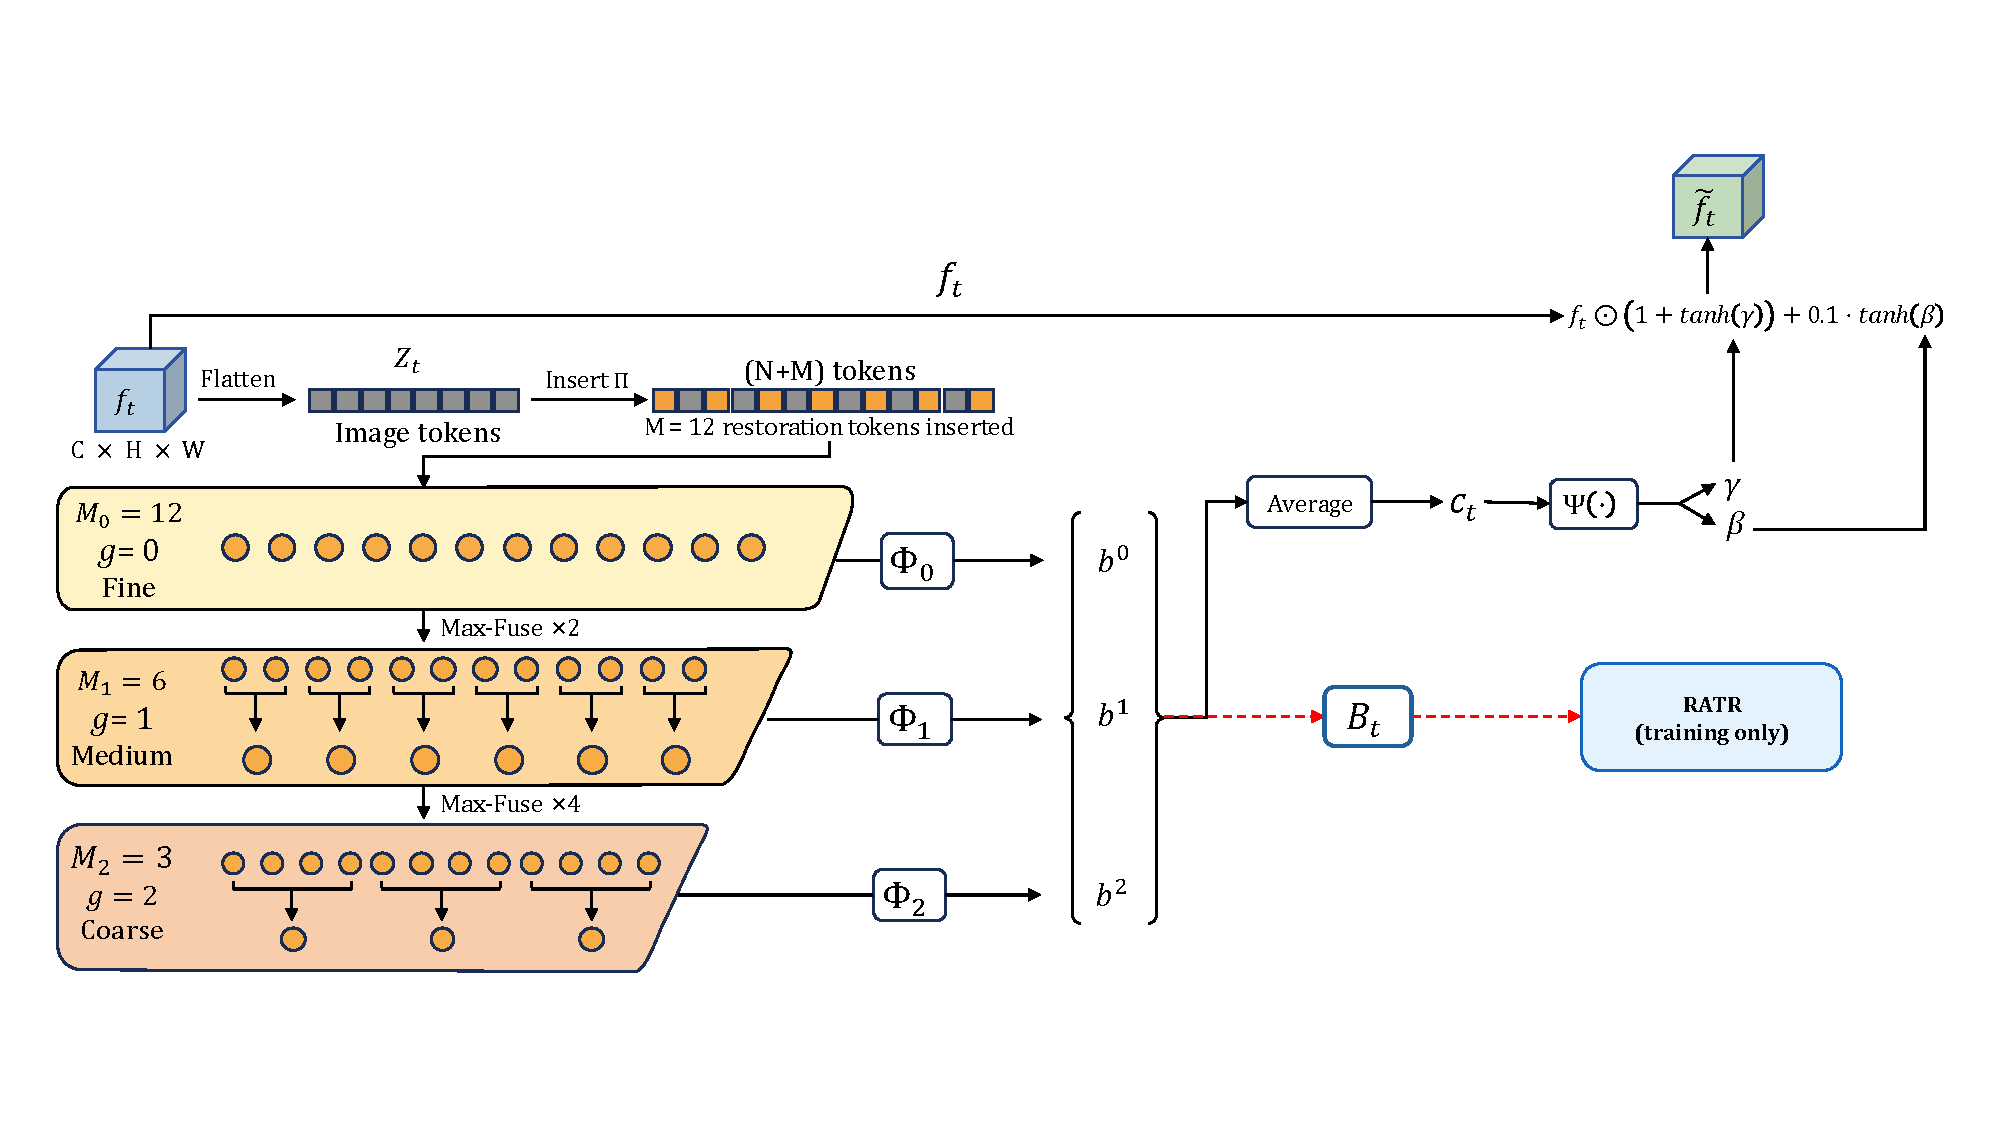
\includegraphics[width=\textwidth]{figures/Fig2_mgfe_module_detail.pdf}
\caption{MGFE module. $M{=}12$ learnable restoration tokens are inserted into image tokens, fused by progressive max fusion, and summarized into $G{=}3$ restoration-token branches. The resulting descriptors generate scale and shift parameters for channel-wise recalibration.\label{fig:mgfe_detail}}
\end{figure}

Since MGFE processes each propagation direction identically, we drop the direction superscript $d$ and write $f_t \in \mathbb{R}^{C_f \times H \times W}$ for brevity. We first flatten it into an image-token sequence

\begin{equation}
Z_t = \operatorname{Flat}(f_t) \in \mathbb{R}^{N \times C_f},
\qquad
N = H W,
\end{equation}

where $\operatorname{Flat}(\cdot)$ preserves raster order and stacks spatial positions into token form. We then append $M$ learnable restoration tokens $R \in \mathbb{R}^{M \times C_f}$ and insert them into the image-token stream through an operator $\Pi(\cdot,\cdot)$:

\begin{equation}
\widehat{Z}_t = \Pi(Z_t, R) \in \mathbb{R}^{(N+M)\times C_f}.
\end{equation}

The insertion operator $\Pi$ distributes restoration tokens uniformly across the image-token stream. It partitions the $N$ image tokens into $M{+}1$ approximately equal chunks and places one restoration token after each of the first $M$ chunks while preserving raster order. Each chunk receives $\lfloor N/(M{+}1)\rfloor$ or $\lceil N/(M{+}1)\rceil$ image tokens so that the total remains exactly $N$. For example, with $M=3$ and $N=9$, the four chunks contain $\{3,2,2,2\}$ image tokens, and the three restoration tokens are inserted at cumulative positions $\{3,6,9\}$ within the 12-token interleaved sequence. This deterministic interleaving gives restoration tokens balanced coverage over the full spatial support.

MGFE builds $G$ granularity branches by progressively fusing restoration tokens. The fusion scheme follows ReIDMamba~\cite{gu2025reidmamba} and is adapted here to propagated spatial restoration features. To make every branch well defined, the number of restoration tokens must satisfy the divisibility constraint
\begin{equation}
M = k \cdot 2^{G-1},\quad k \in \mathbb{N}^{+},
\end{equation}
so that every branch size $M_g = M/2^g$ is an integer for $g\in\{0,\ldots,G-1\}$. We use $G=3$ and $M=12$ ($k=3$) throughout; see Section~\ref{subsec:sensitivity} for alternative configurations.

For branch $g \in \{0,\ldots,G-1\}$, MGFE fuses restoration tokens with a sampling rate of $2^g$. The fused restoration tokens are defined as

\begin{equation}
R^{(g)}[j] =
\mathcal{F}\!\left(
\left\{R[j{\cdot}2^g+k]\right\}_{k=0}^{2^g-1}
\right),\quad
j = 0,\ldots,M_g-1,
\end{equation}

where $\mathcal{F}(\cdot)$ denotes an element-wise maximum operator over all tokens in the fusion group:

\begin{equation}
\mathcal{F}\!\left(
\left\{R[j\cdot2^g+k]\right\}_{k=0}^{2^g-1}
\right)
= \max_{0\le k < 2^g}\,R[j\cdot2^g+k]\;\in\mathbb{R}^{C_f}.
\label{eq:max_fusion}
\end{equation}

The max operation is taken channel-wise. We choose max fusion rather than mean fusion because restoration tokens are intended to retain salient degradation evidence such as scratches, cracks, and blotch boundaries. Mean fusion can dilute sparse high-contrast activations within a group, whereas max fusion preserves the strongest activation in each channel. This design follows ReIDMamba~\cite{gu2025reidmamba}, which reports that max fusion outperforms mean fusion for progressive token aggregation in multi-granularity architectures. Smaller $g$ values preserve more tokens and retain finer local detail, while larger $g$ values compress wider support and emphasize coarse restoration context.

The fused tokens are re-inserted into the same image-token sequence using the same uniform-spacing insertion rule:

\begin{equation}
\widehat{Z}_t^{(g)} = \Pi\!\left(Z_t,R^{(g)}\right),
\end{equation}

and the resulting sequence is processed by a lightweight branch-specific token mixer $\Phi_g(\cdot)$:

\begin{equation}
U_t^{(g)} = \Phi_g\!\left(\widehat{Z}_t^{(g)}\right)
\in \mathbb{R}^{(N+M_g)\times C_f},
\end{equation}

where $M_g = M/2^g$. Each $\Phi_g$ consists of two sequential linear-complexity token blocks. Each block contains a context-augmented projection sublayer and a feed-forward sublayer. The projection sublayer applies LayerNorm, computes a global context vector by mean pooling over the token dimension, adds the projected context to the per-token linear projection, and applies a residual connection. The feed-forward sublayer applies LayerNorm followed by a two-layer MLP with GELU activation and hidden dimension $2C_f$, again with a residual connection. Formally, for input tokens $\mathbf{h}$, each block computes
\begin{equation}
\mathbf{h}' = \mathbf{h} + W_t\,\mathrm{LN}(\mathbf{h}) + W_c\,\overline{\mathrm{LN}(\mathbf{h})},\qquad
\mathbf{h}'' = \mathbf{h}' + \mathrm{MLP}(\mathrm{LN}(\mathbf{h}')),
\end{equation}
where $\overline{(\cdot)}$ denotes mean pooling over the token dimension, $W_t,W_c\in\mathbb{R}^{C_f\times C_f}$ are learned projections, and MLP consists of $\mathrm{Linear}(C_f\!\rightarrow\!2C_f)\!\rightarrow\!\mathrm{GELU}\!\rightarrow\!\mathrm{Linear}(2C_f\!\rightarrow\!C_f)$. The global context term $W_c\,\overline{\mathrm{LN}(\mathbf{h})}$ gives each token a lightweight full-sequence summary at linear cost, avoiding the quadratic complexity of self-attention while retaining inter-token communication. Each branch has its own pair of token blocks, allowing branch-specific parameterization with modest overhead.

After branch processing, MGFE summarizes each branch by averaging the updated restoration-token positions:

\begin{equation}
b_t^{(g)} =
\frac{1}{M_g}
\sum_{m=1}^{M_g}
U_t^{(g)}[\pi_m^{(M_g)}]
\in \mathbb{R}^{D},
\end{equation}

where $\{\pi_m^{(M_g)}\}_{m=1}^{M_g}$ denote the uniformly spaced insertion positions for $M_g$ tokens, and $D=C_f$. Stacking all branch descriptors gives

\begin{equation}
B_t =
\left[
b_t^{(0)}, b_t^{(1)}, \ldots, b_t^{(G-1)}
\right]^\top
\in \mathbb{R}^{G \times D}.
\end{equation}

Because the descriptors are extracted from a common propagated feature under different token-fusion rates, they share semantic alignment while differing in granularity. This descriptor tensor $B_t$ is the input to RATR.

MGFE also converts the branch descriptors into a channel-wise recalibration signal. We first average the branch context,

\begin{equation}
c_t = \frac{1}{G}\sum_{g=0}^{G-1}b_t^{(g)},
\qquad
[\boldsymbol{\gamma}_t,\boldsymbol{\beta}_t] = \Psi(c_t),
\label{eq:recalibration_context}
\end{equation}

where $\Psi(\cdot)$ is a projection head consisting of $\mathrm{LayerNorm}\!\rightarrow\!\mathrm{Linear}(C_f\!\rightarrow\!2C_f)\!\rightarrow\!\mathrm{GELU}\!\rightarrow\!\mathrm{Linear}(2C_f\!\rightarrow\!2C_f)$ that outputs concatenated scale and shift vectors. The recalibrated propagated feature is then

\begin{equation}
\widetilde{f}_t =
f_t \odot
\left(1+\tanh(\boldsymbol{\gamma}_t)\right)
+ 0.1\,\tanh(\boldsymbol{\beta}_t),
\label{eq:recalibration}
\end{equation}

where the vectors in Equation~\eqref{eq:recalibration_context} are broadcast over spatial dimensions. The multiplicative term $(1+\tanh(\boldsymbol{\gamma}_t))$ keeps scaling close to unity at initialization, and the additive coefficient $0.1$ limits the shift magnitude. The shift coefficient $0.1$ bounds the additive term to at most $10\%$ of the $\tanh$ range, keeping the modulation within a conservative $10\%$ shift scale. This conservative FiLM-style modulation~\cite{perez2018film} helps the recalibrated feature remain close to the original propagated feature when the branch context is uncertain. Once the branch descriptors become informative, coarse branches can supply global structural preferences and fine branches can emphasize localized damage patterns.

In summary, MGFE separates restoration evidence by spatial granularity through lightweight token mixing while preserving the baseline interface through residual-style recalibration. The branch descriptors $B_t$ and the recalibration signal $(\boldsymbol{\gamma}_t, \boldsymbol{\beta}_t)$ serve two different roles: the descriptors provide ranking targets for RATR (Section~\ref{subsec:ratr}), while the recalibration feeds granularity-aware modulation back into the propagated feature. This separation allows ablation studies to disable recalibration while keeping branch descriptors active for diversity regularization (see the RATR-only configuration in Section~\ref{subsec:ablation}). Explicit branches alone, however, do not guarantee complementary features. If all branches induce the same sample rankings, branch balance degenerates into redundant descriptors. This motivates the training regularizer described next.

\subsection{Ranking-Aware Triplet Regularization (RATR)}
\label{subsec:ratr}

RATR discourages branch collapse by penalizing excessive ranking correlation between branches. A simple diversity loss could force descriptors to be orthogonal, but orthogonality does not ensure that branches organize restoration evidence differently across samples. The relevant behavior is the branch-specific similarity order induced when an anchor frame is compared with nearby positives and harder negatives. If different branches rank the same candidates identically, they remain redundant even if their descriptor values differ. RATR therefore formulates diversity as an anchor-centered ranking problem using Kendall's~\cite{kendall1938measure} rank correlation coefficient, made differentiable by DiffKendall~\cite{zheng2023diffkendall}. Figure~\ref{fig:ratr_detail} illustrates the workflow.

\begin{figure}[!htbp]
\centering
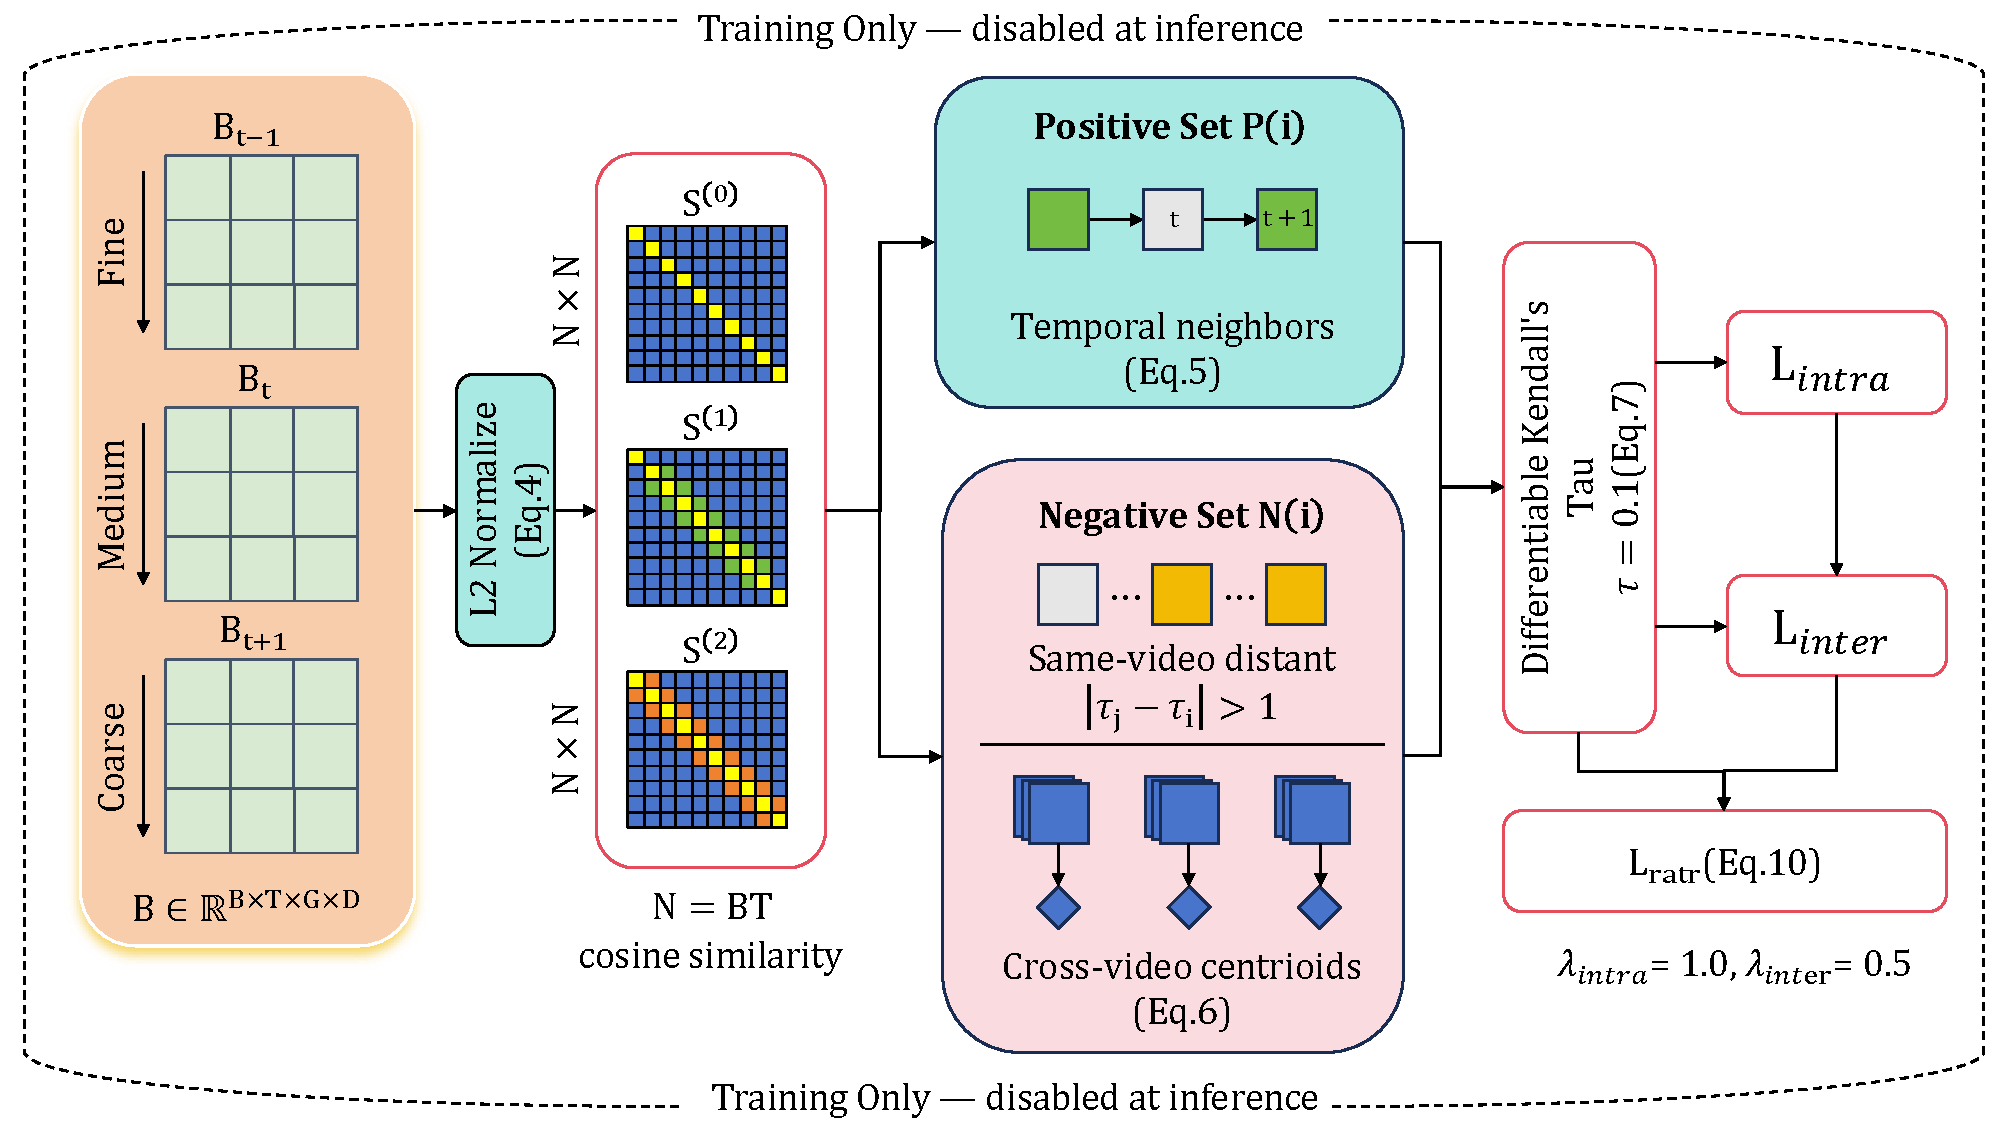
\includegraphics[width=\textwidth]{figures/Fig3_ratr_module_detail.pdf}
\caption{RATR module. Differentiable Kendall's Tau compares branch-specific ranking sequences from temporal correspondences. Neighbor frames define positives, while distant same-video frames and cross-video centroids define negatives, producing $\mathcal{L}_{\text{intra}}$ and $\mathcal{L}_{\text{inter}}$ during training only.\label{fig:ratr_detail}}
\end{figure}

Let the averaged branch descriptors from Equation~\eqref{eq:mgfrofr_overview_2} be organized as a 4D tensor of shape $N_b\times T\times G\times D$, where $N_b$ is the batch size. We flatten batch and time into $\bar{N}=N_b T$ samples and normalize the descriptors branch-wise:

\begin{equation}
\widehat{b}_i^{(g)} =
\frac{b_i^{(g)}}{\|b_i^{(g)}\|_2},
\qquad
i=1,\ldots,\bar{N}.
\end{equation}

For each branch $g$, we compute a cosine-similarity matrix

\begin{equation}
\mathcal{S}^{(g)}[i,j] =
\left\langle
\widehat{b}_i^{(g)},
\widehat{b}_j^{(g)}
\right\rangle.
\end{equation}

This matrix is not used as a standalone supervision target. Instead, it provides the positive and negative ranking sequences that form the anchor-positive-negative structure regularized by RATR.

For anchor $i$, the positive set is defined from temporal correspondences within the same clip:

\begin{equation}
\mathcal{P}(i)=
\bigl\{
j \mid v_j=v_i,\;
|t_j-t_i|=1
\bigr\},
\end{equation}

where $v_i$ and $t_i$ denote the clip index and frame index of sample $i$. This temporal adjacency criterion is justified because the flow-guided deformable alignment in MambaOFR has already warped neighboring frames toward the anchor frame before MGFE is applied. After this alignment, adjacent frames are the most reliable proxy for true flow-based correspondences in the feature domain. Since $|\mathcal{P}(i)| \le 2$, boundary frames provide only one positive neighbor. We therefore evaluate the intra-ranking term only on anchors with at least two positives:
\begin{equation}
\mathcal{I}_{\text{intra}}=
\bigl\{
i \mid |\mathcal{P}(i)| \ge 2
\bigr\}.
\end{equation}
For the seven-frame clips used in training, this excludes only the first and last frame of each clip. Interior anchors then contribute exactly one pairwise ordering comparison to $\mathcal{L}_{\text{intra}}$. This limited signal is sufficient in practice because (i)~$\mathcal{L}_{\text{intra}}$ is averaged over many valid anchors in each batch, and (ii)~$\mathcal{L}_{\text{inter}}$ supplies a complementary ranking signal from the richer negative set.

Negative evidence is drawn from two harder sources: temporally distant frames inside the same clip and clip-level representatives from other clips. The same-video negatives are

\begin{equation}
\mathcal{N}_{sv}(i)=
\bigl\{
j \mid v_j=v_i,\;
|t_j-t_i|>1
\bigr\},
\end{equation}

and the clip-level centroid for another video $v\neq v_i$ is

\begin{equation}
\bar{b}_{v}^{(g)} =
\frac{1}{|\mathcal{T}_v|}
\sum_{t\in\mathcal{T}_v}
\widehat{b}_{(v,t)}^{(g)},
\end{equation}

where $\mathcal{T}_v$ denotes the set of frame indices in clip $v$. We then construct the negative ranking sequence as

\begin{equation}
\bar{\mathcal{S}}_i^{(g)} =
\Bigl[\mathcal{S}^{(g)}[i,j]\Bigr]_{j\in\mathcal{N}_{sv}(i)}
\oplus
\Bigl[\bigl\langle \widehat{b}_i^{(g)},\,\bar{b}_v^{(g)} \bigr\rangle\Bigr]_{v\neq v_i},
\end{equation}

where $\oplus$ denotes sequence concatenation. Same-video distant frames are hard negatives because they share content and degradation statistics with the anchor but are no longer immediate temporal neighbors. Off-video centroids provide a low-variance clip-level representative that avoids the $O(\bar{N}^2)$ cost of enumerating every cross-clip frame pair while still capturing inter-clip distributional contrast.

To compare how two branches rank the same candidate set, we adopt a differentiable version of Kendall's Tau. For sequences $p,q\in\mathbb{R}^{L}$, the differentiable statistic is

\begin{equation}
\mathrm{DKTau}(p,q;\tau)
= \frac{1}{\binom{L}{2}}
\sum_{1\le u < v \le L}
\tanh\!\!\left(\frac{p_u-p_v}{\tau}\right)
\cdot
\tanh\!\!\left(\frac{q_u-q_v}{\tau}\right),
\label{eq:dktau}
\end{equation}

where $\tau>0$ is a temperature parameter. As $\tau\rightarrow 0$, Equation~\eqref{eq:dktau} approaches the hard sign comparison used in the exact Kendall coefficient; as $\tau$ becomes too large, pairwise order differences are oversmoothed and gradients vanish. We set $\tau=0.1$ (see Section~\ref{subsec:sensitivity} for the sensitivity to this choice). A lower value of $\mathrm{DKTau}(p,q;\tau)$ indicates weaker ranking correlation between branches and therefore stronger branch complementarity.

Using Equation~\eqref{eq:dktau}, we compute the positive-ranking correlation loss as

\begin{equation}
\mathcal{L}_{\text{intra}} =
\frac{1}{|\mathcal{I}_{\text{intra}}| \binom{G}{2}}
\sum_{i\in\mathcal{I}_{\text{intra}}}
\sum_{g < g'}
\mathrm{DKTau}\!\Bigl(
\mathcal{S}^{(g)}[i,\mathcal{P}(i)],\,
\mathcal{S}^{(g')}[i,\mathcal{P}(i)];\,\tau
\Bigr),
\label{eq:loss_intra}
\end{equation}

and the negative-ranking correlation loss as

\begin{equation}
\mathcal{L}_{\text{inter}} =
\frac{1}{\bar{N} \binom{G}{2}}
\sum_{i=1}^{\bar{N}}
\sum_{g < g'}
\mathrm{DKTau}\!\Bigl(
\bar{\mathcal{S}}_i^{(g)},\,
\bar{\mathcal{S}}_i^{(g')};\,
\tau
\Bigr).
\end{equation}

The final ranking-aware regularizer is

\begin{equation}
\mathcal{L}_{\text{ratr}} =
\lambda_{\text{intra}}\,\mathcal{L}_{\text{intra}}
+ \lambda_{\text{inter}}\,\mathcal{L}_{\text{inter}}.
\label{eq:loss_ratr}
\end{equation}

Equations~\eqref{eq:loss_intra}--\eqref{eq:loss_ratr} play complementary roles. The intra term prevents two branches from assigning nearly identical orders to the most likely temporal correspondences, while the inter term prevents the same collapse on harder negatives. Minimizing both terms does not force arbitrary disagreement because the restoration losses still anchor the recalibrated feature stream to the reconstruction target through MGFE.

\subsection{Training Objective}
\label{subsec:training_objective}

The generator objective combines the standard OFR losses used by the MambaOFR baseline with the proposed ranking-aware regularizer. Specifically, we use an $L_1$ pixel reconstruction loss $\mathcal{L}_{\mathrm{pix}}$, whose robustness for image restoration objectives is analyzed in~\cite{zhao2017loss_restoration}, a VGG-based perceptual loss $\mathcal{L}_{\mathrm{perc}}$~\cite{johnson2016perceptual}, an adversarial loss $\mathcal{L}_{\mathrm{gan}}$~\cite{goodfellow2014gan}, and the proposed ranking regularization $\mathcal{L}_{\mathrm{ratr}}$:

\begin{equation}
\mathcal{L}_{\mathrm{total}} =
\mathcal{L}_{\mathrm{pix}}
+ \lambda_{\mathrm{perc}}\mathcal{L}_{\mathrm{perc}}
+ \lambda_{\mathrm{gan}}\mathcal{L}_{\mathrm{gan}}
+ \lambda_{\mathrm{ratr}}\mathcal{L}_{\mathrm{ratr}}.
\label{eq:loss_total}
\end{equation}

Equation~\eqref{eq:loss_total} preserves backward compatibility with the baseline training loop because MGFE only augments the propagated feature stream and RATR appears purely as an auxiliary regularizer. The loss weights are set to $\lambda_{\mathrm{perc}}=1.0$ and $\lambda_{\mathrm{gan}}=0.01$, following RTN~\cite{wan2022rtn} and MambaOFR~\cite{mao2025mambaofr}. For the ranking term, we use $\lambda_{\mathrm{ratr}}=0.1$, $\lambda_{\mathrm{intra}}=1.0$, and $\lambda_{\mathrm{inter}}=0.5$ (see Section~\ref{subsec:sensitivity} for sensitivity to these choices). The smaller weight on $\mathcal{L}_{\text{inter}}$ reflects the coarser ordering signal of clip-centroid negatives. Unless otherwise stated, the full model uses feature dimension $C_f=16$, $G=3$ branches, $M=12$ restoration tokens, channel-wise max fusion in Equation~\eqref{eq:max_fusion}, and a differentiable Kendall temperature of $\tau=0.1$.
